%!TEX root = SISC_elastic_3d.tex
\subsection{LOH.1 model problem with layered material}
As the final numerical example, we consider the LOH.1 model problem. It has a layered material model where the top $1000$ meters ($z\in[0,1000]$) has different properties than the rest of the domain. The computational domain is taken to be $(x,y,z)\in[0,30000]^2\times[0,17000]$. The dynamic and mechanical parameters are given in Table \ref{material_parameter}. The problem is driven by a single point moment source. The moment tensor $M$ has one element $M_{xy} = 1e18$ and other elements are $0$. The position of the source is in the lower half-space at the point $(x,y,z) = (15000, 15000, 2000)$. The time function for the source function is a Gaussian given by
\[g(t,t_0,\omega) = \frac{\omega}{\sqrt{2\pi}}e^{-\omega^2(t - t_0)^2/2}, \ \ \ \omega = 16.6667,\ \ \ \ t_0 = 0.36.\]

\begin{table}[htbp]
	\begin{center}
		\begin{tabular}{c c c c c}
			\hline
			~   & Depth $[m]$& $V_p[m/s]$ & $V_s [m/s]$ & $\rho[Kg/m^3]$ \\
			\hline
			Layer&0--1000& 4000& 2000& 2600\\
			Lower half-space &1000--17000 & 6000 & 3464& 2700\\
			\hline 
		\end{tabular}
	\end{center}
	\caption{Dynamic and mechanical parameters for the layer and the lower half-space of the layer over half-space test.}\label{material_parameter}
\end{table} 

We solve the LOH.1 model problem by using the open source code SW4, where our proposed method has been implemented. The solution is recorded in a receiver on the free surface at the point $(x, y, z) = (21000, 23000, 0)$. And the vertical, transverse and radial velocities time histories are shown in Figure \ref{loh1_100} with $h = 100$ for the lower half-space, $h/2 = 50$ for the layer space; in Figure \ref{loh1_50} with $h = 50$ for the lower half-space, $h/2 = 25$ for the layer space. From Figure \ref{loh1_100} and Figure \ref{loh1_50} , we observe that our method does not generate any artifacts as $h$ become small enough.
\begin{figure}[htbp]
	\centering
	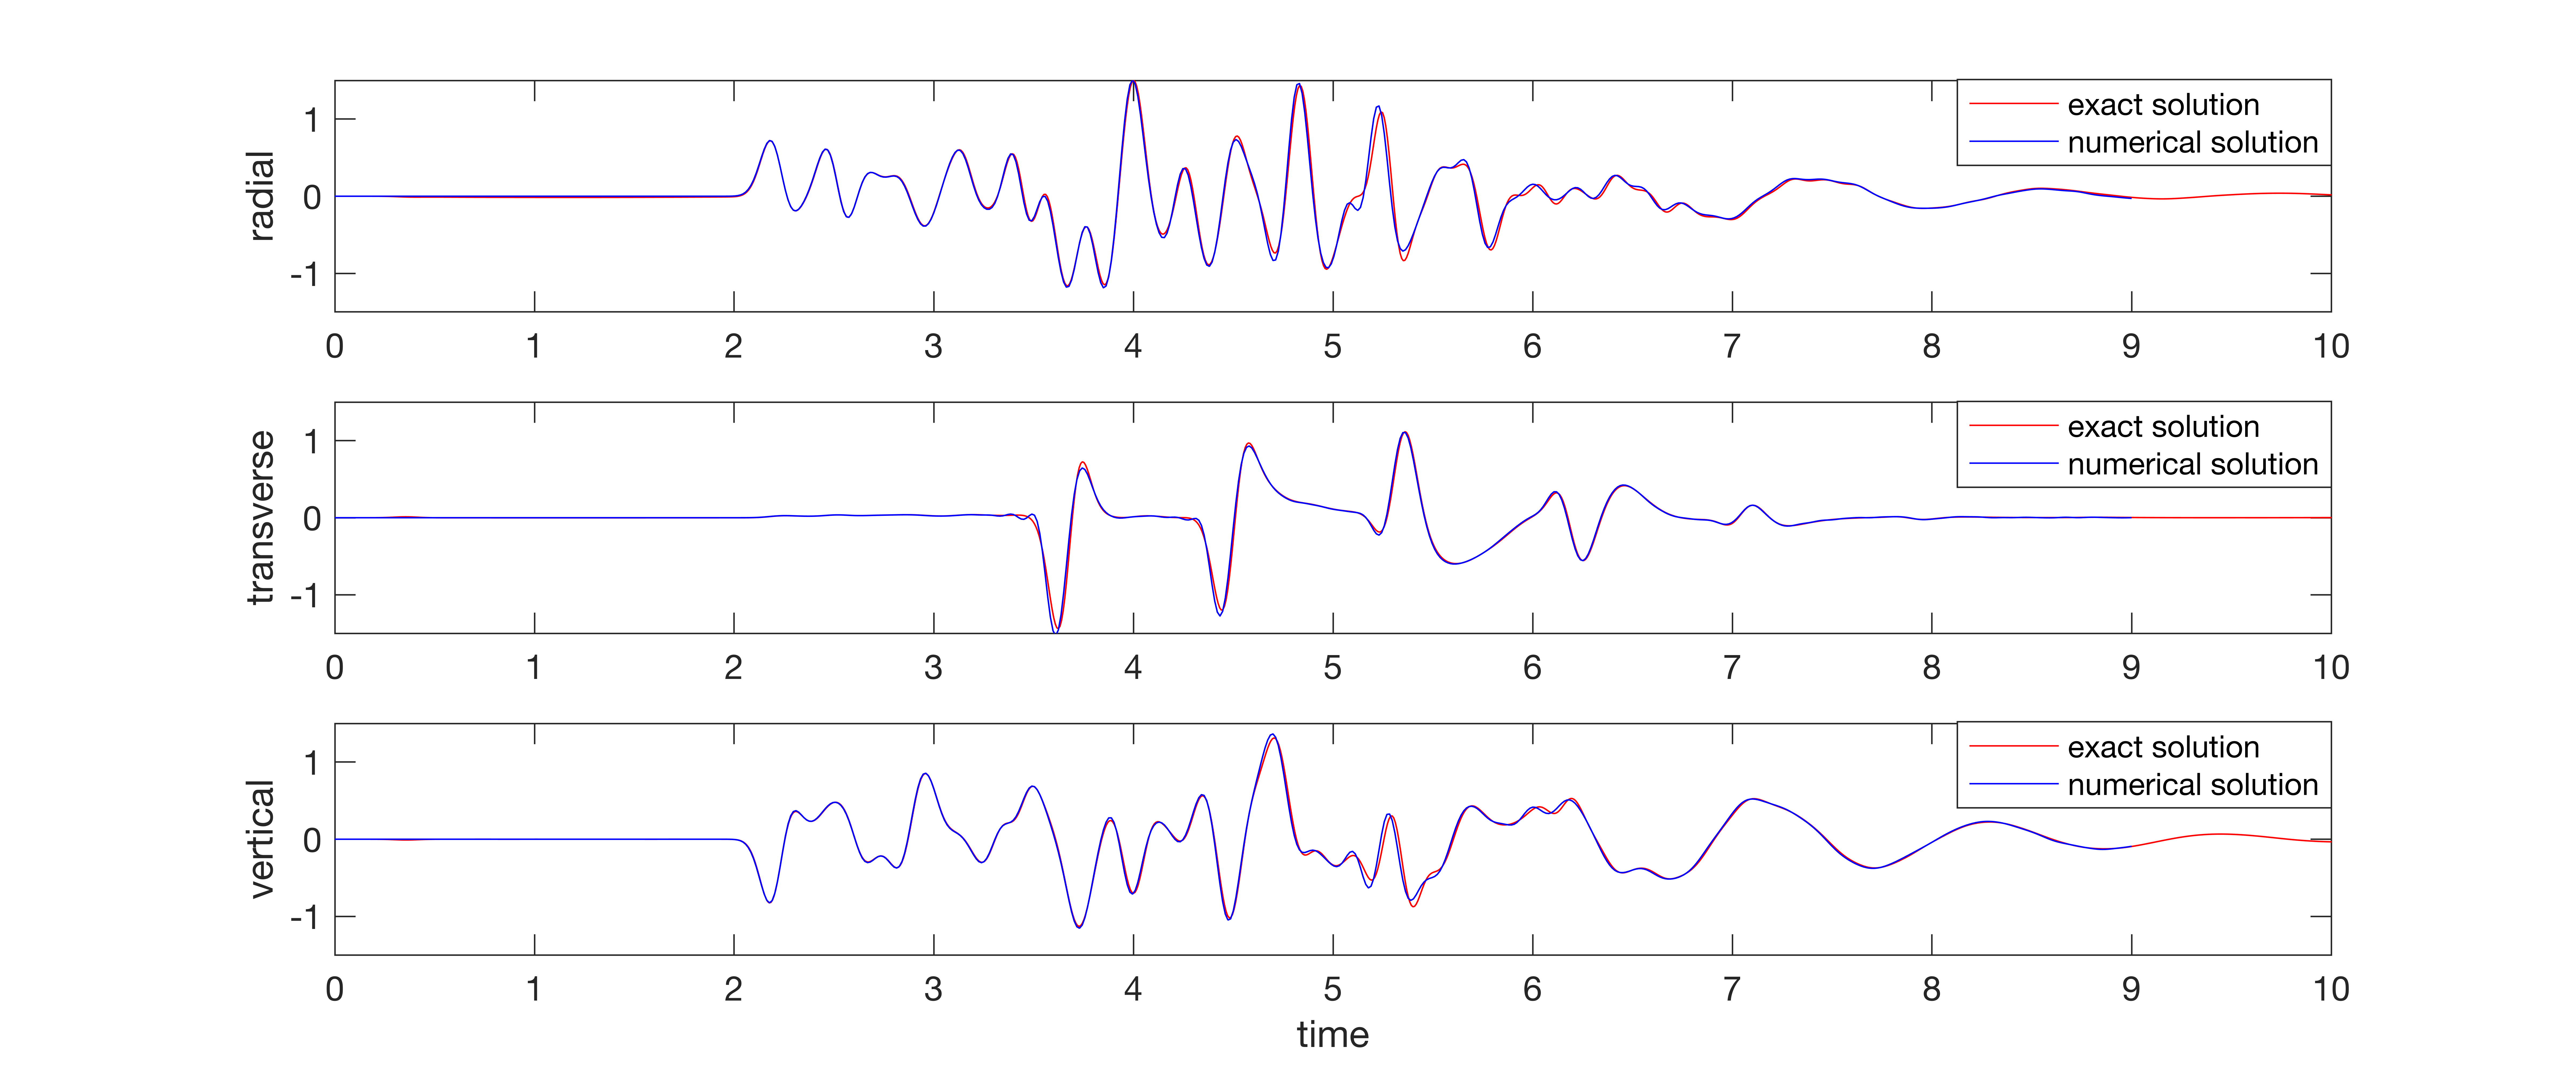
\includegraphics[width=0.9\textwidth,trim={2cm 0cm 2cm 0cm}, clip]{loh1_h100.png}
	\caption{LOH.1: The radial (top), transverse (middle), and vertical (bottom) velocities time histories. Here the numerical solutions are plotted in blue ($h = 100$) and the semi-analytical solution is plotted in red.}\label{loh1_100}
\end{figure}

\begin{figure}[htbp]
	\centering
	\includegraphics[width=0.9\textwidth,trim={2cm 0cm 2cm 0cm}, clip]{loh1_h50.png}
	\caption{LOH.1: The radial (top), transverse (middle), and vertical (bottom) velocities time histories. Here the numerical solutions are plotted in blue ($h = 50$) and the semi-analytical solution is plotted in red.}\label{loh1_50}
\end{figure}

To test the performance of the new method, we record the quotient between the computational time of the time-stepping procedure and of solving the linear system for the mesh refinement interface in Table \ref{time}. We have run simulations on two different computer clusters. First, we use two nodes on the Rackham cluster with each node consisting of two 10-core Intel Xeon V4 CPUs and 128 GB memory. We also use three nodes on ManeFrame II (M2) with each node consisting of two 18-core Intel Xeon E5-2695 v4 CPUs and 256 GB memory. From Table \ref{time}, we observe that our new method which only uses ghost points from the coarse domain needs less time on solving interface conditions compared with the old method in SW4 which uses ghost points from both coarse and fine domains.

\begin{table}[htbp]
	\begin{center}
		\begin{tabular}{|c|c|c|}
			\hline
			Machine   & new method & odd method \\
			\hline
			Rackham & 4.02\% &  8.16\%\\
			\hline
			M2 &5.17\% & 8.87\%\\
			\hline 
		\end{tabular}
	\end{center}
		\caption{MR time / time-stepping time}\label{time}
\end{table} 


